\documentclass[a4paper,12pt]{article}

\usepackage[T1]{fontenc}
\usepackage{geometry}
\geometry{
    total={150mm,237mm},
    left=30mm,
    top=30mm,
}
\usepackage{amsmath}
\usepackage{multicol}

\usepackage{tikz}
\usepackage{tkz-euclide}

\setlength{\parindent}{0pt}

\begin{document}
% \large
\section*{Geometric Proof for Pythagoras' Theorem}

You might be familiar with Pythagoras' theorem for right angled
triangles. where for a right angled triangle with sides $a$, $b$, 
and $c$, where $c$ is the hypotenuse we know that 
$$c^2 = a^2 + b^2.$$
But can we be convinced that this is in fact true?

\subsection*{Setup}
First let there be a generic right angled triangle with side lengths
$a$, $b$, and $c$ wwith $c$ as the hypotenuse.

\begin{figure}[h]
\centering
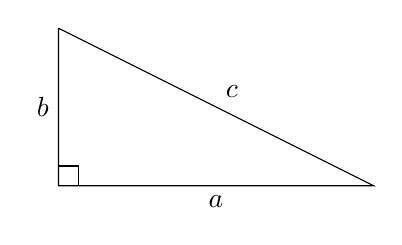
\begin{tikzpicture}
    \coordinate (C) at (0, 0);
    \coordinate (B) at (4, 0);
    \coordinate (A) at (0, 2);
    
    \draw (A) -- node[left] {$b$} (C)
        -- node[below] {$a$} (B)
        -- node[above right] {$c$} (A);
    \tkzMarkRightAngle(A,C,B)
\end{tikzpicture}
\end{figure}

From this four of these triangles we can construct a square.

\begin{figure}[h]
\centering
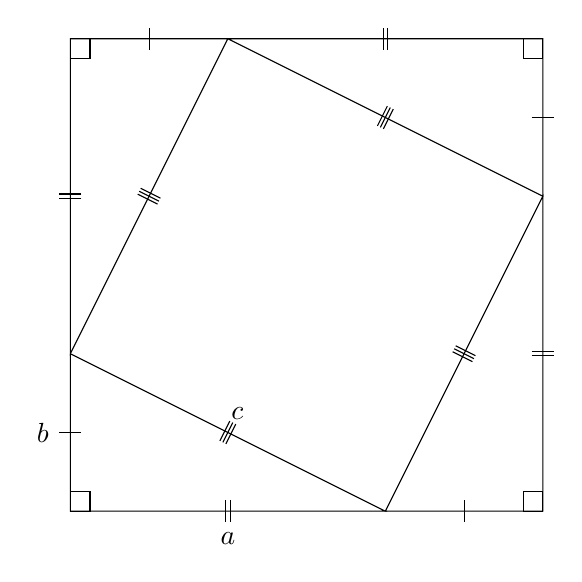
\begin{tikzpicture}
    \coordinate (A1) at (0, 2);
    \coordinate (C1) at (0, 0);
    \coordinate (A2) at (4, 0);
    \coordinate (C2) at (6, 0);
    \coordinate (A3) at (6, 4);
    \coordinate (C3) at (6, 6);
    \coordinate (A4) at (2, 6);
    \coordinate (C4) at (0, 6);
    
    \draw (A1) -- node[left=0.15cm] {$b$} (C1)
        -- node[below=0.15cm] {$a$} (A2)
        -- node[above right,pos=0.52] {$c$} (A1);
    \tkzMarkRightAngle(A1,C1,A2)
    \tkzMarkSegment[pos=0.5,mark=|](C1,A1)
    \tkzMarkSegment[pos=0.5,mark=||](C1,A2)
    \tkzMarkSegment[pos=0.5,mark=|||](A1,A2)

    \draw (A2) -- (C2) -- (A3) -- cycle;
    \tkzMarkSegment[pos=0.5,mark=|](A2,C2)
    \tkzMarkSegment[pos=0.5,mark=||](C2,A3)
    \tkzMarkSegment[pos=0.5,mark=|||](A2,A3)
    \tkzMarkRightAngle(A2,C2,A3)
    \draw (A3) -- (C3) -- (A4) -- cycle;
    \tkzMarkSegment[pos=0.5,mark=|](A3,C3)
    \tkzMarkSegment[pos=0.5,mark=||](C3,A4)
    \tkzMarkSegment[pos=0.5,mark=|||](A3,A4)
    \tkzMarkRightAngle(A3,C3,A4)
    \draw (A4) -- (C4) -- (A1) -- cycle;
    \tkzMarkSegment[pos=0.5,mark=|](A4,C4)
    \tkzMarkSegment[pos=0.5,mark=||](C4,A1)
    \tkzMarkSegment[pos=0.5,mark=|||](A4,A1)
    \tkzMarkRightAngle(A4,C4,A1)
\end{tikzpicture}
\end{figure}

Each side of this square is the $a + b$, this means that the
area of the square is given by $(a + b)^2$. But we can also 
treat the area of the square as 

\end{document}
